%  !TeX spellcheck = en_GB
%  WangSheying于2015/11/2整理,TJU北洋园校区
%  TeXLive2015+TeXstudio个人推荐,可在线升级usepackage,比较方便
%*****************************************************************************************
%  从这里开始到\begin{document}是导言区,称之为preamble
\documentclass[UTF8]{beamer}
\usepackage[fontset=mac]{ctex}
%\usepackage[UTF8]{ctex}                 %使用中文要添加,可解决中文文档输入
\usepackage{newtxtext,newtxmath}  %字重齐全的高质量数学字体
\usepackage{mathrsfs}             %大写ABC的花体使用命令是\mathscr{}
\usepackage{graphicx}             %添加图片
\usepackage{bm}                   %专门处理数学粗体的bm宏包,使用命令是\bm{}
\usepackage{extarrows}            %延长符号,可在=,->等符号加多个字母
%\usepackage{amstext}              %它定义命令 \text,可用于在数学公式中插入少量文本,并可调整上下标中文本字体的尺寸。
\usepackage{amsthm}               %它定义了一个 proof 环境,用来排版定理和证明,能自动在最后添加证毕符号。它还提供一个命令:\newtheorem{定理环境名}{标题}[计数器名],可自定义定理类 环境
\usefonttheme{professionalfonts}  %这个更好看些,数学字体
\usepackage{indentfirst}          %首行缩进
\usepackage{verbatim}
\usepackage{amsmath}
\usepackage{amsfonts}
\usepackage{amssymb}
\usepackage{xcolor}
\usepackage{subfigure}
\usepackage[english]{babel}
\usepackage{algorithm}
\usepackage{algorithmic}
\usepackage{tikz}
\setlength{\parindent}{2em}      %首行缩进2字符
\setbeamertemplate{theorems}[numbered]
\setbeamertemplate{caption}[numbered]
%******************************************************************************************
%            以上是各种宏包
%******************************************************************************************
%下面是定理,定义,引言的声明,可自行添加

\newtheorem{thm}{Theorem}
\newtheorem{lem}[thm]{Lemma}
\newtheorem{cor}[thm]{Corollary}
\newtheorem{prop}[thm]{Proposition}
\newtheorem{defi}[thm]{Definition}
\newtheorem{remark}[thm]{Remark}
\newtheorem{claim}[thm]{Claim}

\newenvironment{proofnoqed}{\begin{proof}<span style="background-color: rgb(255, 0, 0);">\renewcommand{\qedsymbol}{}  }{\end{proof} }
%有的证明比较长,前面的应该没有证毕符号,只在最后一个用proof,其他应该用自定义的新环境proofnoqed



%  三种颜色   red  purple   magenta





%上面是定理,定义,引言的声明,可自行添加
%******************************************************************************************
%下面是beamer的主题设置,目录框架结构,其实就是标题,目录等在上下左右哪一个位置放置,以及目录怎么显示
\usetheme{Singapore}            % 幻灯片模板选择singapore
\usecolortheme{sidebartab}      % 幻灯片模板的色彩sidebartab

\AtBeginSection[]{              % 幻灯片框架% 在每个Section前都会加入的Frame,
	\begin{frame}[plain]
		\frametitle{Outline}
		\tableofcontents[sectionstyle=show/shaded,subsectionstyle=show/show/shaded]
	\end{frame} 
}
%  \tableofcontents[comma-separated option list]具体讲解见《The beamer class User Guide》,
%  http://texdoc.net/texmf-dist/doc/latex/beamer/doc/beameruserguide.pdf     See in section 10.5 Adding a table of contents.
%  section和subsection相互独立,显示效果互不相关,Allowed ⟨styles⟩ are show, shaded, and hide
%  sectionstyle=⟨style for current section⟩/⟨style for other sections⟩
%  subsectionstyle=⟨style for current subsection⟩/⟨style for other subsections in current section⟩/⟨style for subsections in other sections⟩
%
% 上面是beamer的主题设置,目录框架结构,其实就是标题,目录等在上下左右哪一个位置放置,以及目录怎么显示
%*******************************************************************************************
%       下面标题页的内容设置,根据实际情况修改即可
\title{The Design and Implementation of Kafka}  % 幻灯片封面
\author{Wang Sheying}
\institute{HuiLongGuan of Beijing}
\date{\today}  

%\date{9月 23, 2019}%一般是\today
%      上面标题页的内容设置根据实际情况修改即可
%*******************************************************************************************
%  \begin{document}以上是导言区,称之为preamble
%*******************************************************************************************
\begin{document}
	\begin{frame}[plain]
		%plain格式使得一帧的最上面是白色的,没有plain,会有色彩
		\titlepage
	\end{frame}
	\begin{frame}[plain]               % 幻灯片目录
		\frametitle{Outline}
		\tableofcontents[sectionstyle=show/show,subsectionstyle=show/show/hide]
	\end{frame}
	%The beamer class这本小册子有目录格式的讲解,sectionstyle,subsectionstyle都有,P100页
	%User Guide for version 3.36. 文档可在google搜索The beamer class,即可得到
%  以上是标准的配置,还有最下面的一部分标准配置
%********************************************************************************************
%    一帧的具体格式样例参考
%\section{节的名字}
%\subsection{小节的名字}
%\begin{frame}[plain,t]{节的名字} %也可以使用\frametitle{节的名字}效果一样
%	\structure{小节的名字} \\  \vspace{2ex}
%	节的名字正上方居中,小节的名字紧下方居左。
%\end{frame}
%*********************************************************************************************
%                  下面就是正文,自己的内容
%*********************************************************************************************

\section{Introduction}
\begin{frame}[plain,t]{Introduction} %也可以使用\frametitle{节的名字}效果一样
	%\structure{} \\
	  \vspace{2ex}

   Apache Kafka is used for building real-time data pipelines and streaming apps. It is horizontally scalable, fault-tolerant, wicked fast, and runs in production in thousands of companies.
    

\begin{figure}
    \centering
    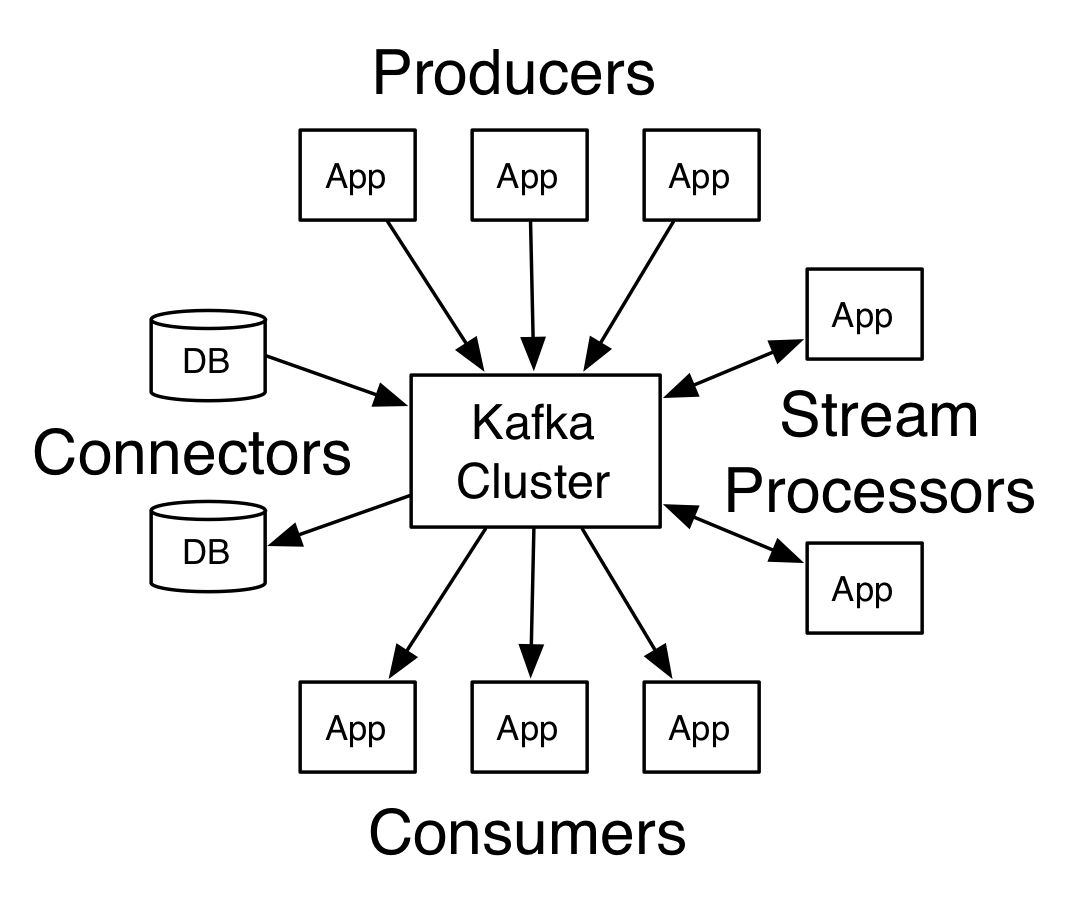
\includegraphics[width=0.7\linewidth]{image/0101}
    %\caption{}
    \label{fig:0101}
\end{figure}
\end{frame}


\begin{frame}[plain,t]{Introduction} %也可以使用\frametitle{节的名字}效果一样
    %\structure{} \\
    \vspace{2ex}
    \begin{figure}
        \centering
        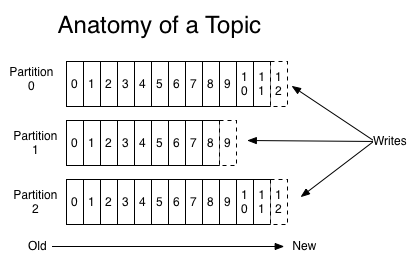
\includegraphics[width=0.8\linewidth]{image/0102}
        %\caption{}
        \label{fig:0102}
    \end{figure}
    
    
 
\end{frame}
\begin{frame}[plain,t]{Introduction} %也可以使用\frametitle{节的名字}效果一样
    %\structure{} \\
    \vspace{2ex}
    \begin{figure}
        \centering
        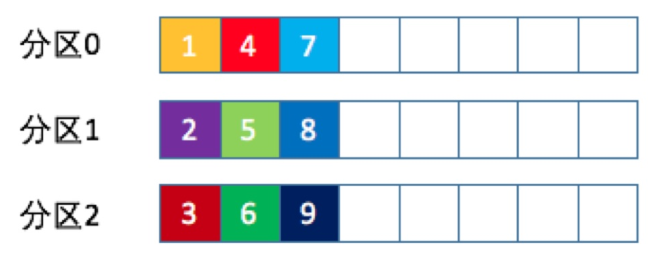
\includegraphics[width=0.8\linewidth]{image/0105}
        %\caption{}
        \label{fig:0105}
    \end{figure}
    
    
    
\end{frame}
\begin{frame}[plain,t]{Introduction} %也可以使用\frametitle{节的名字}效果一样
    %\structure{} \\
    \vspace{2ex}
     \begin{figure}
        \centering
        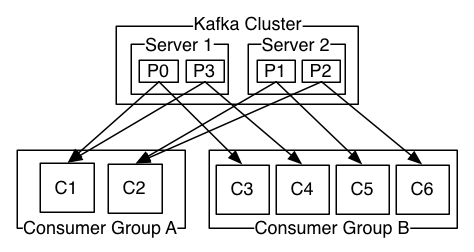
\includegraphics[width=0.9\linewidth]{image/0103}
        %\caption{}
        \label{fig:0103}
    \end{figure}
    
    
    
    
\end{frame}
\begin{frame}[plain,t]{Introduction} %也可以使用\frametitle{节的名字}效果一样
    %\structure{} \\
    \vspace{2ex}
    
     \begin{figure}
        \centering
        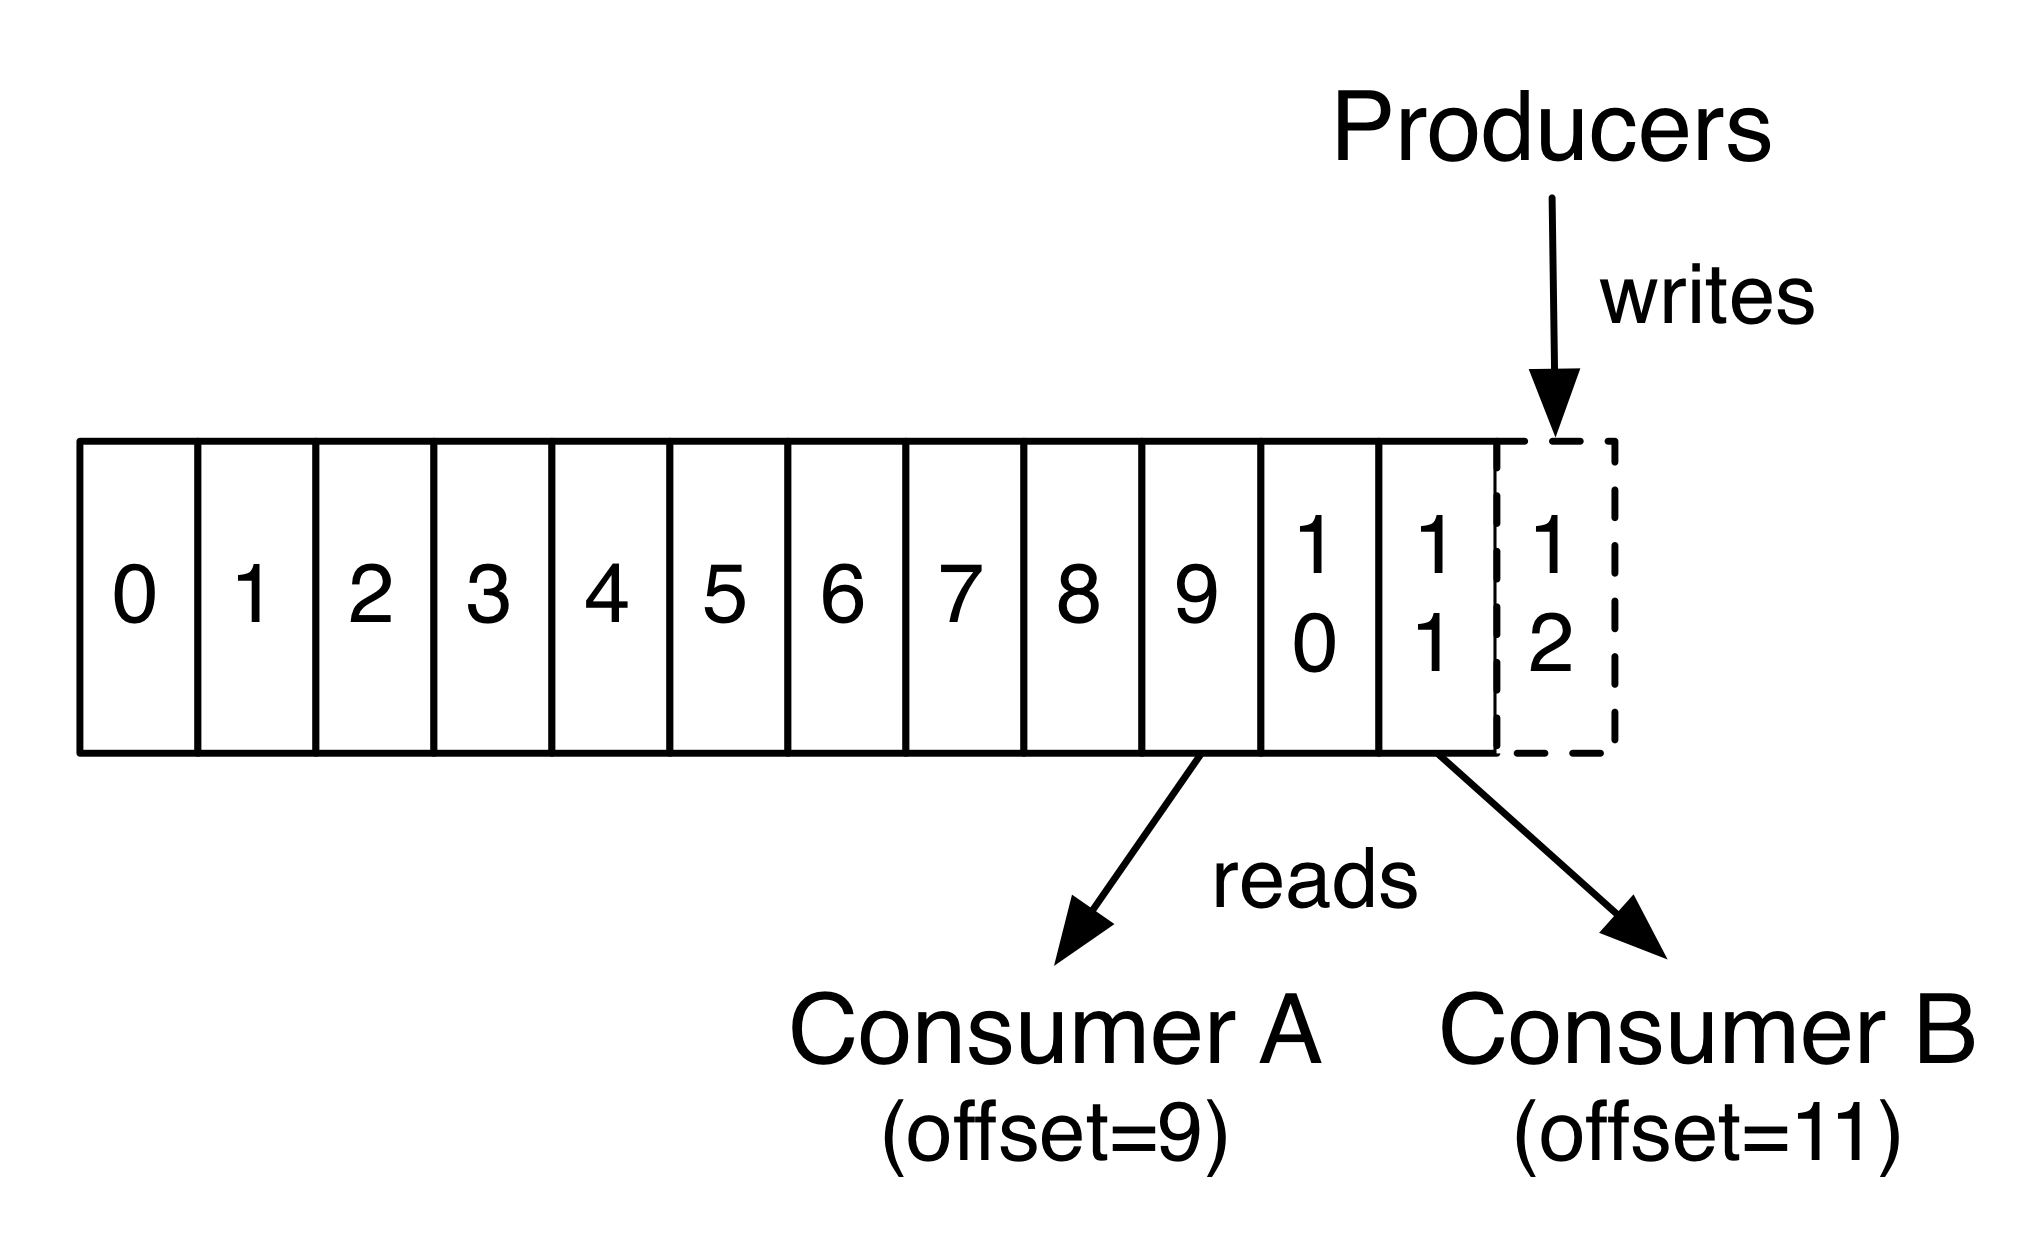
\includegraphics[width=0.9\linewidth]{image/0104}
        %\caption{}
        \label{fig:0104}
    \end{figure}
    
    
    
\end{frame}
\section{Design}
\subsection{Persistence}
\begin{frame}[plain,t]{Design} %也可以使用\frametitle{节的名字}效果一样
    \structure{Persistence} \\
    \vspace{2ex}
    Kafka relies heavily on the filesystem for storing and caching messages. 
    
    \begin{figure}
        \centering
        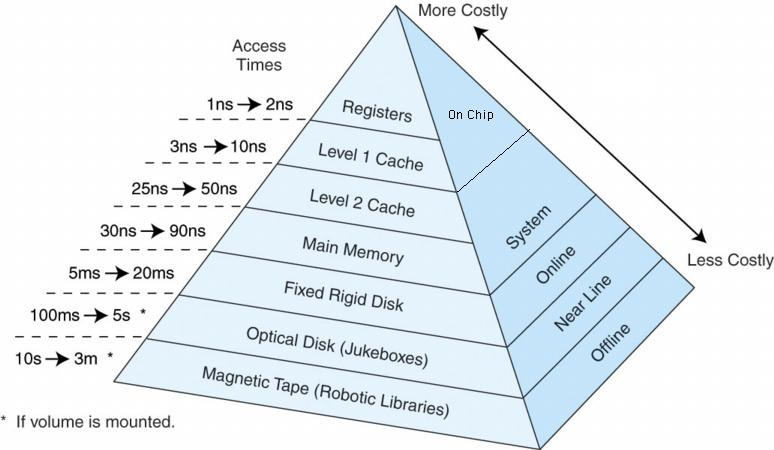
\includegraphics[width=0.8\linewidth]{image/0212}
        %\caption{}
        \label{fig:0212}
    \end{figure}
    
    
    
\end{frame}
\subsection{Efficiency}
\begin{frame}[plain,t]{Design} %也可以使用\frametitle{节的名字}效果一样
    \structure{Efficiency} \\
    \vspace{2ex}
   As a result the performance of linear writes on a JBOD configuration with six 7200rpm SATA RAID-5 array is about 600MB/sec but the performance of random writes is only about 100k/sec—a difference of over 6000X. 
   
   \vspace{2ex}
   \begin{figure}
       \centering
       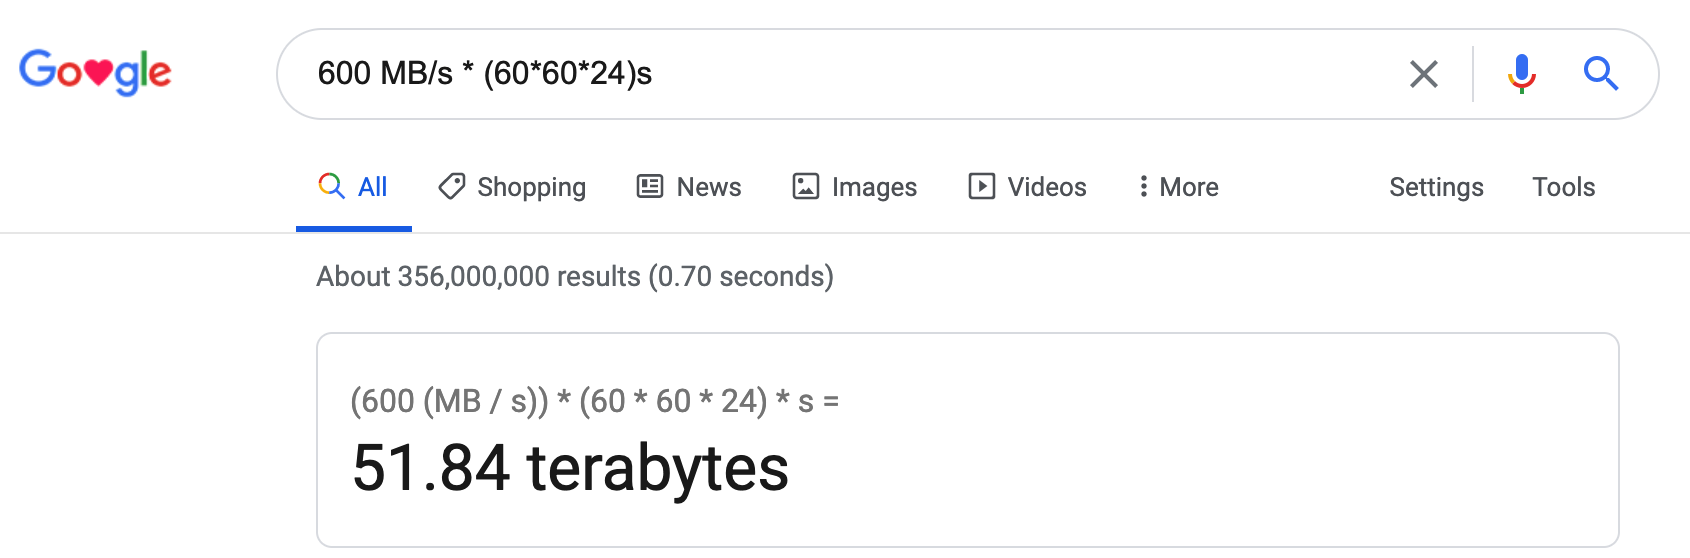
\includegraphics[width=0.9\linewidth]{image/0213}
       %\caption{}
       \label{fig:0213}
   \end{figure}
   
   
   %\vspace{2ex}
   %To compensate for this performance divergence, modern operating systems have become increasingly aggressive in their use of main memory for disk caching.
   
    
    
\end{frame}
\begin{frame}[plain,t]{Design} %也可以使用\frametitle{节的名字}效果一样
    \structure{Efficiency} \\
    \vspace{2ex}
The killer when working with a disk? Access time. Today, a page fault stalls the CPU for millions of cycles; as clock speeds increase, this penalty will increase to tens of millions of cycles.

 \vspace{2ex}
 This is why caching data in memory({\color{red}page cache}) is so important for performance – disk is 5 orders of magnitude slower than RAM.

%To address the gap, %between memory and disk access times
 %we will prefetch data from the Personal Terabyte magnetic disk into {\color{red}page cache}.

   \vspace{2ex}
     The modern OS predicts future accesses based on past access patterns and then performs a cost-benefit analysis to determine whether the benefit of prefetching a block exceeds its cost.
    

    
    
\end{frame}
\begin{frame}[plain,t]{Design} %也可以使用\frametitle{节的名字}效果一样
    \structure{Efficiency} \\
    \vspace{2ex}
   
    To illustrate the page cache, I'll conjure a Linux program named render, which opens file scene.dat and reads it 512 bytes at a time, storing the file contents into a heap-allocated block. 
    
   \begin{figure}
       \centering
       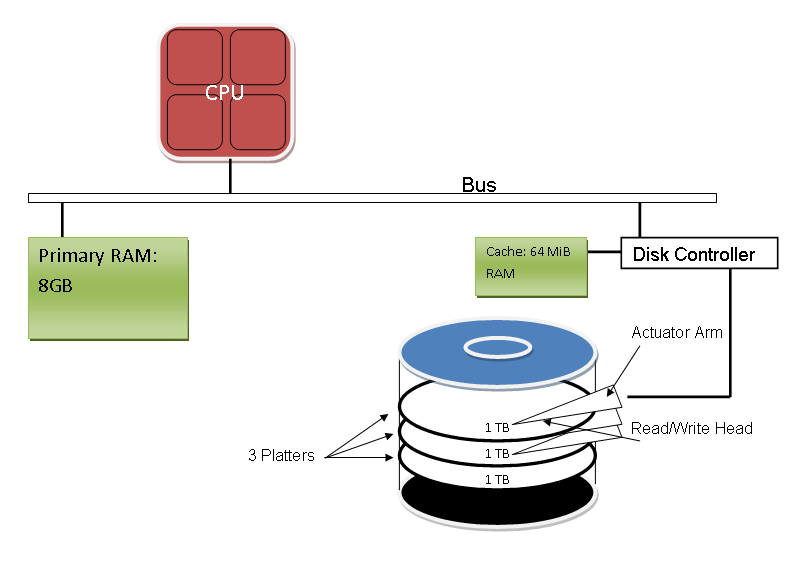
\includegraphics[width=0.7\linewidth]{image/0214}
       %\caption{}
       \label{fig:0214}
   \end{figure}

   %the difference in latency between RAM and a hard drive is enormous.
   
   %This type of prefetching will be essential to achieving high performance on the Personal Terabyte.
   %To avoid an I/O bottleneck, we must prefetch disk data into memory so that it is available to the processor without incurring a page fault. 
   
   
  %We are performing a prefetching study that 
 
   
    
    
\end{frame}
\begin{frame}[plain,t]{Design} %也可以使用\frametitle{节的名字}效果一样
    \structure{Efficiency} \\
    \vspace{2ex}
    The first read goes like this:
    \begin{figure}
        \centering
        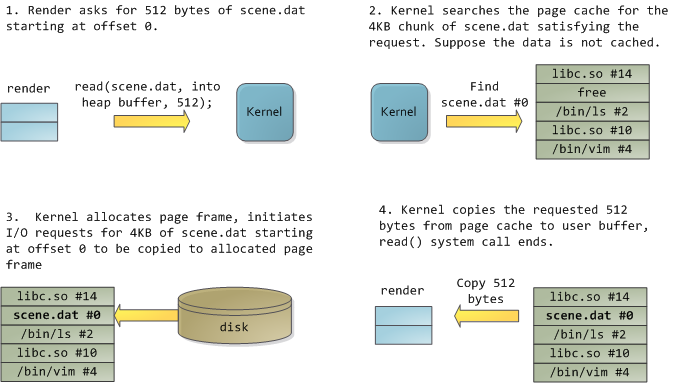
\includegraphics[width=0.9\linewidth]{image/0215}
        %\caption{}
        \label{fig:0215}
    \end{figure}
    
\end{frame}
\begin{frame}[plain,t]{Design} %也可以使用\frametitle{节的名字}效果一样
    \structure{Efficiency} \\
    \vspace{2ex}
    When you use {\color{red}memory-mapped files}, the kernel maps your program's virtual pages directly onto the page cache.
    
    \vspace{2ex}
    \begin{figure}
        \centering
        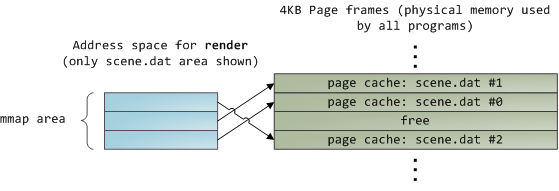
\includegraphics[width=0.9\linewidth]{image/0216}
        %\caption{}
        \label{fig:0216}
    \end{figure}
    
\end{frame}
\begin{frame}[plain,t]{Design} %也可以使用\frametitle{节的名字}效果一样
    \structure{Efficiency} \\
    \vspace{2ex}
    
    All disk reads and writes will go through this unified cache. 
    
    \vspace{2ex}
    So long as there's enough free physical memory, the cache should be kept full. It is therefore not dependent on a particular process, but rather it's a system-wide resource. 
    
    %A modern operating system provides read-ahead and write-behind techniques that prefetch data in large block multiples and group smaller logical writes into large physical writes.
    
    \vspace{2ex}
    A modern OS will happily divert all free memory to disk caching with little performance penalty when the memory is reclaimed.
    
    
    
\end{frame}
\begin{frame}[plain,t]{Design} %也可以使用\frametitle{节的名字}效果一样
    \structure{Efficiency} \\
    \vspace{2ex}
    Furthermore, kafka are building on top of the JVM, and anyone who has spent any time with Java memory usage knows two things:
    \vspace{2ex}
    \begin{itemize}
        \item The memory overhead of objects is very high.
        \item  Java garbage collection becomes increasingly fiddly and slow as the in-heap data increases.
    \end{itemize}
    
    
   
    
    
\end{frame}
\begin{frame}[plain,t]{Design} %也可以使用\frametitle{节的名字}效果一样
    \structure{Efficiency} \\
    \vspace{2ex}
    As a result of these factors using the filesystem and relying on pagecache is superior to maintaining an in-memory cache or other structure.
    
    \vspace{2ex}
    Doing so will result in a cache of up to 28-30GB on a 32GB machine without GC penalties.
    
    \vspace{2ex}
   % Furthermore, this cache will stay warm even if the service is restarted, whereas the in-process cache will need to be rebuilt in memory
    All data is immediately written to a persistent log on the filesystem without necessarily flushing to disk.
    
    %This suggests a design which is very simple: rather than maintain as much as possible in-memory and flush it all out to the filesystem in a panic when we run out of space, we invert that. 
    
    \vspace{2ex}
    %All data is immediately written to a persistent log on the filesystem without necessarily flushing to disk.
    
    \vspace{2ex}
    %In effect this just means that it is transferred into the kernel's pagecache.
    
\end{frame}

\begin{frame}[plain,t]{Design} %也可以使用\frametitle{节的名字}效果一样
    \structure{Efficiency} \\
    \vspace{2ex}
    The persistent data structure used in messaging systems are often a per-consumer queue with an associated BTree or other general-purpose random access data structures to maintain metadata about messages.
    
    \vspace{2ex}
    They do come with a fairly high cost, though: Btree operations are O(log N). Normally O(log N) is considered essentially equivalent to constant time, but this is not true for disk operations. 
    
    \vspace{2ex}
    Since storage systems mix very fast cached operations with very slow physical disk operations, the observed performance of tree structures is often superlinear as data increases with fixed cache.
    
    
    
\end{frame}
\begin{frame}[plain,t]{Design} %也可以使用\frametitle{节的名字}效果一样
    \structure{Efficiency} \\
    \vspace{2ex}
    Intuitively a persistent queue could be built on simple reads and appends to files as is commonly the case with logging solutions. 
    
    \vspace{2ex}
    This structure has the advantage that all operations are O(1) and reads do not block writes or each other. 
    
    \vspace{2ex}
    This has obvious performance advantages since the performance is completely decoupled from the data size.
    
    
    
\end{frame}

\begin{frame}[plain,t]{Design} %也可以使用\frametitle{节的名字}效果一样
    \structure{Efficiency} \\
    \vspace{2ex}
    We assume each message published is read by at least one consumer (often many), hence we strive to make consumption as cheap as possible.
    
    \vspace{2ex}
    Once poor disk access patterns have been eliminated, there are two common causes of inefficiency in this type of system:%: too many small I/O operations, and excessive byte copying.
    \begin{itemize}
        \item too many small I/O operations
        \item excessive byte copying
    \end{itemize}
    
    
    
\end{frame}
\begin{frame}[plain,t]{Design} %也可以使用\frametitle{节的名字}效果一样
    \structure{Efficiency} \\
    \vspace{2ex}
    The small I/O problem happens both between the client and the server and in the server's own persistent operations.
    
    \vspace{2ex}
    To avoid this, our protocol is built around a "message set" abstraction that naturally groups messages together. 
    
   
    %This allows network requests to group messages together and amortize the overhead of the network roundtrip rather than sending a single message at a time. 
    \vspace{2ex}
    The server in turn appends chunks of messages to its log in one go, and the consumer fetches large linear chunks at a time.
    
    
    
    
\end{frame}
\begin{frame}[plain,t]{Design} %也可以使用\frametitle{节的名字}效果一样
    \structure{Efficiency} \\
    \vspace{2ex}
    This simple optimization produces orders of magnitude speed up. 
    
    \vspace{2ex}
    Batching leads to larger network packets, larger sequential disk operations, contiguous memory blocks, and so on.
    
    \vspace{2ex}
    All of which allows Kafka to turn a bursty stream of random message writes into linear writes that flow to the consumers.
    
    
    
    
\end{frame}
\begin{frame}[plain,t]{Design} %也可以使用\frametitle{节的名字}效果一样
    \structure{Efficiency} \\
    \vspace{2ex}
    The other inefficiency is in byte copying.
    
    \vspace{2ex}
    To avoid this we employ a standardized binary message format that is shared by the producer, the broker, and the consumer,so data chunks can be transferred without modification between them.
    
     \vspace{2ex}
     
     The message log maintained by the broker is itself just a directory of files, each populated by a sequence of message sets that have been written to disk in the same format used by the producer and consumer. 
    
    
    
    
\end{frame}
\begin{frame}[plain,t]{Design} %也可以使用\frametitle{节的名字}效果一样
    \structure{Efficiency} \\
   
    \vspace{2ex}
    Maintaining this common format allows optimization of the most important operation: network transfer of persistent log chunks. 
    
    \vspace{2ex}
    Modern unix operating systems offer a highly optimized code path for transferring data out of pagecache to a socket; in Linux this is done with the sendfile system call.
    
     \vspace{2ex}
    The Java class libraries support zero copy on Linux and UNIX systems through  java.nio.channels.FileChannel.transferTo(). 
    
    
    
\end{frame}
\begin{frame}[plain,t]{Design} %也可以使用\frametitle{节的名字}效果一样
    \structure{Efficiency} \\
    \vspace{2ex}
    To understand the impact of sendfile, it is important to understand the common data path for transfer of data from file to socket:
    \begin{enumerate}
        \item The operating system reads data from the disk into pagecache in kernel space
        \item The application reads the data from kernel space into a user-space buffer
        \item The application writes the data back into kernel space into a socket buffer
        \item The operating system copies the data from the socket buffer to the NIC buffer where it is sent over the network
    \end{enumerate}
    
\end{frame}
\begin{frame}[plain,t]{Design} %也可以使用\frametitle{节的名字}效果一样
    \structure{Efficiency} \\
    \vspace{-1ex}
    \begin{figure}
        \centering
        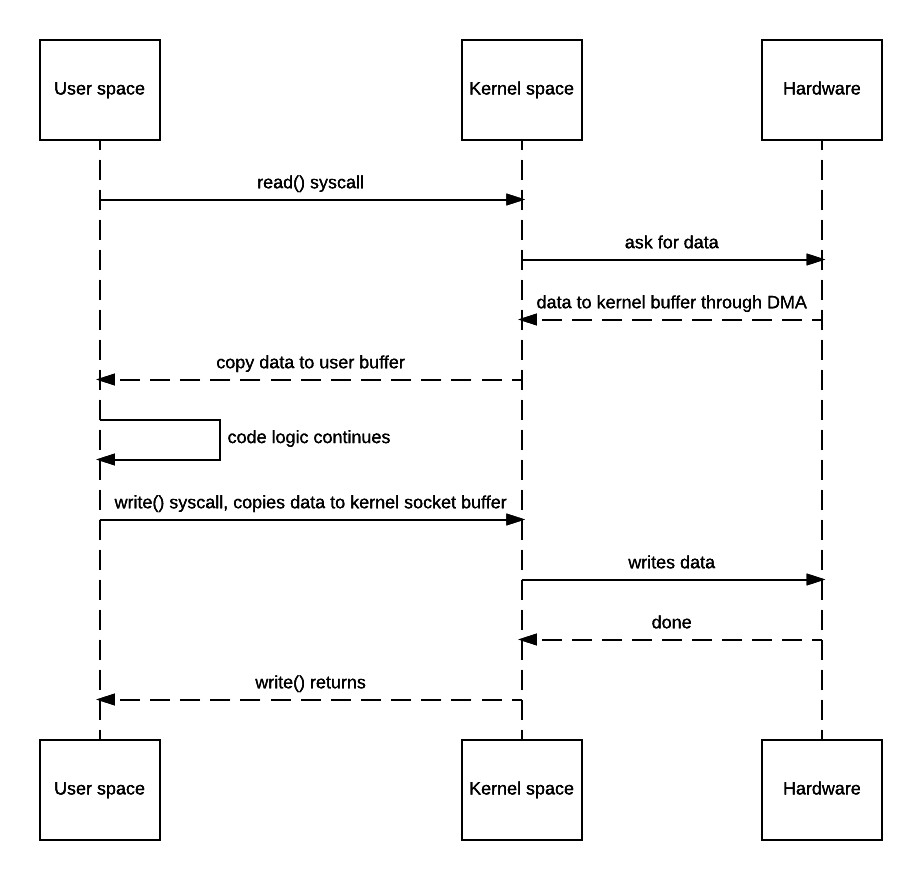
\includegraphics[width=0.7\linewidth]{image/0201}
        %\caption{}
        \label{fig:0201}
    \end{figure}
    
    
    
\end{frame}

\begin{frame}[plain,t]{Design} %也可以使用\frametitle{节的名字}效果一样
    \structure{Efficiency} \\
    \vspace{2ex}
    This is clearly inefficient, there are four copies and two system calls. 
    
    \vspace{2ex}
    Using sendfile, this re-copying is avoided by allowing the OS to send the data from pagecache to the network directly. 
    
    \vspace{2ex}
    So in this optimized path, only the final copy to the NIC buffer is needed.
    
\end{frame}
\begin{frame}[plain,t]{Design} %也可以使用\frametitle{节的名字}效果一样
    \structure{Efficiency} \\
    \vspace{-1ex}
    \begin{figure}
        \centering
        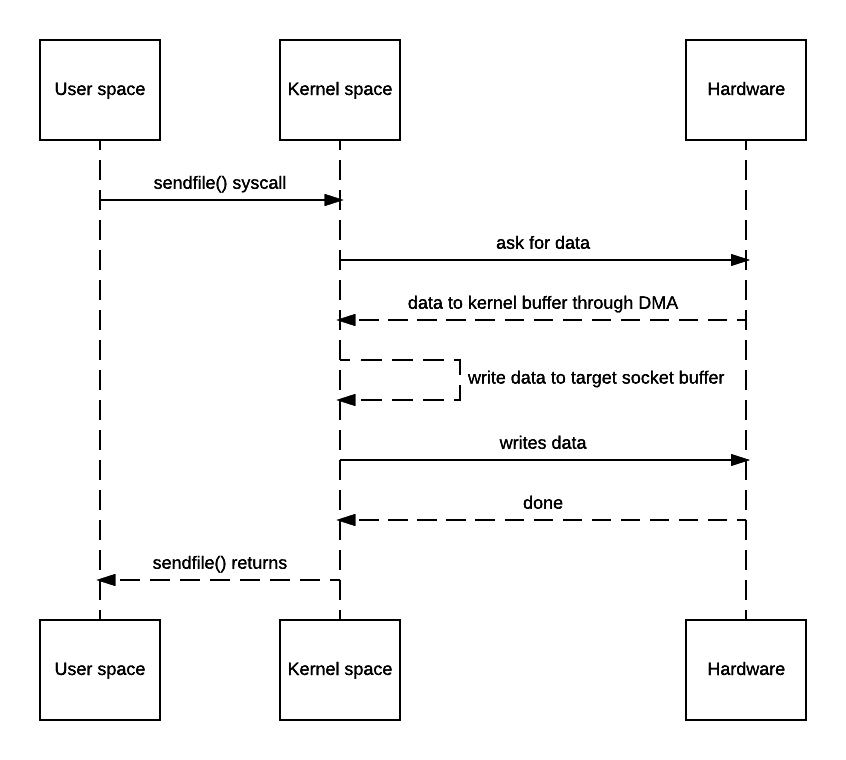
\includegraphics[width=0.7\linewidth]{image/0202}
        %\caption{}
        \label{fig:0202}
    \end{figure}
    
    
\end{frame}


\begin{frame}[plain,t]{Design} %也可以使用\frametitle{节的名字}效果一样
    \structure{Efficiency} \\
    \vspace{2ex}
    Using the zero-copy optimization above, data is copied into pagecache exactly once and reused on each consumption. % instead of being stored in memory and copied out to user-space every time it is read. 
    
    \vspace{2ex}
    This allows messages to be consumed at a rate that approaches the limit of the network connection.
    
    \vspace{2ex}
    This combination of pagecache and sendfile means that on a Kafka cluster 
    %where the consumers are mostly caught up 
    you will see no read activity on the disks whatsoever as they will be serving data entirely from cache.
    
\end{frame}
\begin{frame}[plain,t]{Design} %也可以使用\frametitle{节的名字}效果一样
    \structure{Efficiency} \\
    \vspace{2ex}
    In some cases the bottleneck is actually not CPU or disk but network bandwidth.
    
    \vspace{2ex}
    Efficient compression requires compressing multiple messages together rather than compressing each message individually.
    
    \vspace{2ex}
    Kafka supports this with an efficient batching format. 
    
\end{frame}
\begin{frame}[plain,t]{Design} %也可以使用\frametitle{节的名字}效果一样
    \structure{Efficiency} \\
    \vspace{2ex}
    A batch of messages can be clumped together compressed and sent to the server in this form. 
    
    \vspace{2ex}
    This batch of messages will be written in compressed form and will remain compressed in the log and will only be decompressed by the consumer.
    
    \vspace{2ex}
    Kafka supports GZIP, Snappy, LZ4 and ZStandard compression protocols.
    
    
\end{frame}

\subsection{The Producer}
\begin{frame}[plain,t]{Design} %也可以使用\frametitle{节的名字}效果一样
    \structure{The Producer} \\
    \vspace{2ex}
    The producer sends data directly to the broker that is the leader for the partition without any intervening routing tier. 
    
    \vspace{2ex}
    To help the producer do this all Kafka nodes can answer a request for metadata 
    %about which servers are alive and where the leaders for the partitions of a topic are 
    at any given time to allow the producer to appropriately direct its requests.
    
     \vspace{2ex}
    The client controls which partition it publishes messages to.
    
    
\end{frame}
\begin{frame}[plain,t]{Design} %也可以使用\frametitle{节的名字}效果一样
    \structure{The Producer} \\
    \vspace{2ex}
    Batching is one of the big drivers of efficiency, and to enable batching the Kafka producer will attempt to accumulate data in memory and to send out larger batches in a single request. 
    
    \vspace{2ex}
    The batching can be configured to accumulate no more than a fixed number of messages and to wait no longer than some fixed latency bound (say 64k or 10 ms). 
    
    %This allows the accumulation of more bytes to send, and few larger I/O operations on the servers. 
    \vspace{2ex}
    This buffering is configurable and gives a mechanism to trade off a small amount of additional latency for better throughput.
    
    
    
\end{frame}
\begin{frame}[plain,t]{Design} %也可以使用\frametitle{节的名字}效果一样
    \structure{The Producer} \\
    \vspace{2ex}
    \begin{figure}
        \centering
        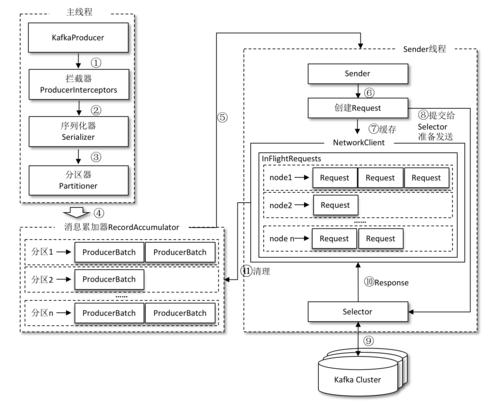
\includegraphics[width=0.7\linewidth]{image/0203}
        %\caption{}
        \label{fig:0203}
    \end{figure}
    
    
    
\end{frame}
\begin{frame}[plain,t]{Design} %也可以使用\frametitle{节的名字}效果一样
    \structure{The Producer} \\
    \vspace{2ex}
    	\begin{center}
        ProducerRecord(Main Thread) \\
        $\Downarrow$ \\
        ProducerBatch (Sender Thread) \\
        $\Downarrow$ \\
        <Partition, Deque<ProducerBatch>{}>(Sender Thread) \\
        $\Downarrow$ \\
        <Node, List<ProducerBatch>{}>(Sender Thread) \\
        $\Downarrow$ \\
        <Node, Request>(Sender Thread) \\
        {\color{red}$\Downarrow$} \\
        Broker(page cache) \\
        $\Downarrow$ \\
        Broker(log segment)
    \end{center}
    
    
\end{frame}
\begin{frame}[plain,t]{Design} %也可以使用\frametitle{节的名字}效果一样
    \structure{The Producer} \\
    \vspace{2ex}
    Kafka provides an asynchronous send method to send a record to a topic.
    
    
    \vspace{1ex}
    \begin{figure}
        \centering
        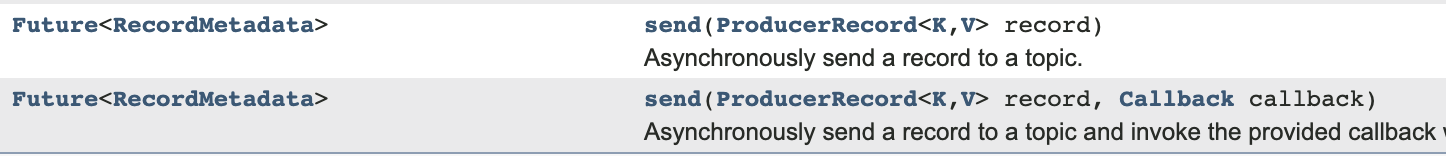
\includegraphics[width=0.9\linewidth]{image/0204}
        %\caption{}
        \label{fig:0204}
    \end{figure}
    
    
    \begin{itemize}
        \item synchronous
        \begin{itemize}
            \item block
            \item Future<RecordMetadata>.get()
        \end{itemize}
        \item asynchronous
        \begin{itemize}
            \item unblock
            \item the callback interface
        \end{itemize}
    \end{itemize}


\end{frame}
\begin{frame}[plain,t]{Design} %也可以使用\frametitle{节的名字}效果一样
    \structure{The Producer} \\
    \vspace{2ex}

  
    If records are sent faster than they can be transmitted to the server then this buffer space will be exhausted. 
    
     \vspace{2ex}
    When the buffer space is exhausted additional send calls will block. 
    
     \vspace{2ex}
    The threshold for time to block is determined by max.block.ms after which it throws a TimeoutException.
    
    
    
\end{frame}
\begin{frame}[plain,t]{Design} %也可以使用\frametitle{节的名字}效果一样
    \structure{The Producer} \\
    \vspace{2ex}
    
    The producer is thread safe and sharing a single producer instance across threads will generally be faster than having multiple instances.
    
    \vspace{2ex}
   From Kafka 0.11, the KafkaProducer supports two additional modes: 
   \begin{itemize}
       \item  the idempotent producer
       \item the transactional producer
   \end{itemize}

    
\end{frame}
\subsection{The Consumer}
\begin{frame}[plain,t]{Design} %也可以使用\frametitle{节的名字}效果一样
    \structure{The Consumer} \\
    \vspace{2ex}
    The Kafka consumer works by issuing "fetch" requests to the brokers leading the partitions it wants to consume. 
    
    \vspace{2ex}
    The consumer specifies its offset in the log with each request and receives back a chunk of log beginning from that position. 
    
     \vspace{2ex}
   %The consumer thus has significant control over this position and can rewind it to re-consume data if need be.
    \begin{figure}
        \centering
        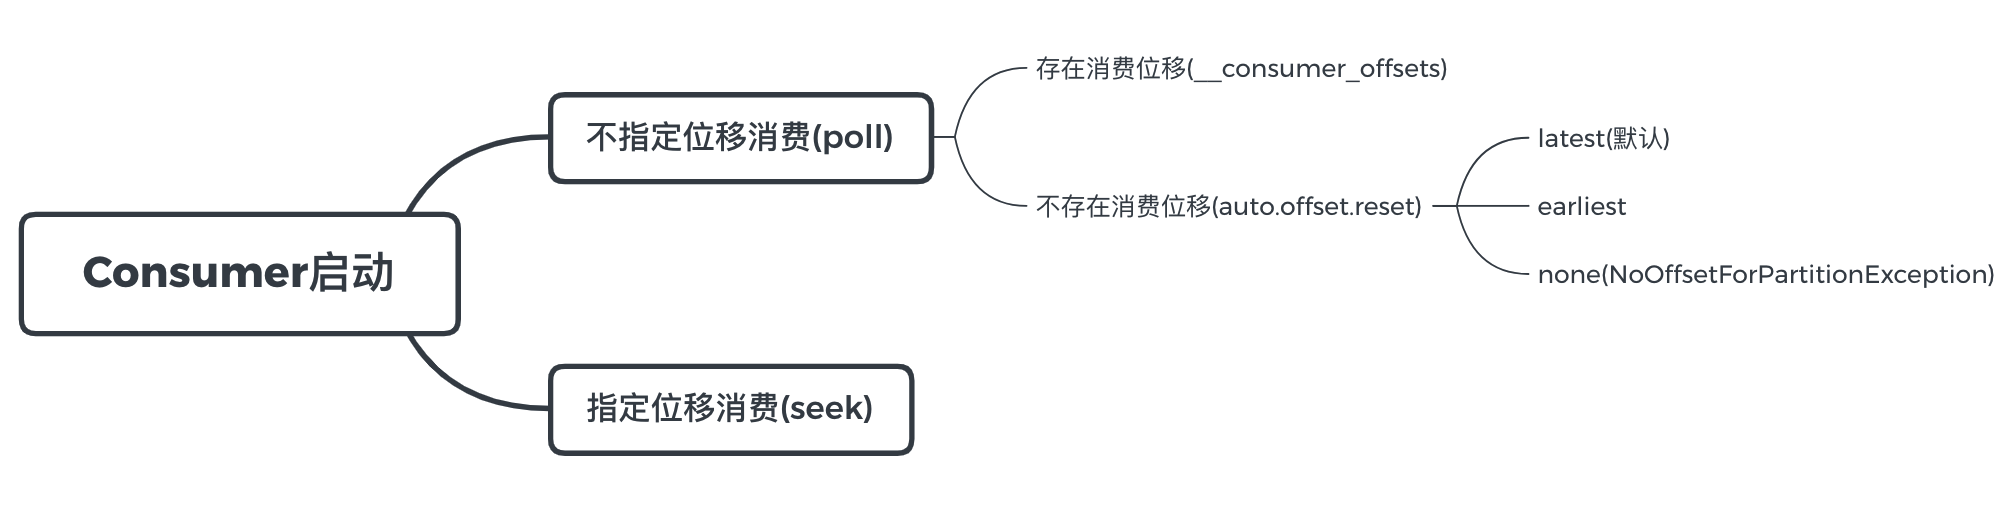
\includegraphics[width=0.9\linewidth]{image/0217}
        %\caption{}
        \label{fig:0217}
    \end{figure}
    
    
\end{frame}

\begin{frame}[plain,t]{Design} %也可以使用\frametitle{节的名字}效果一样
    \structure{The Consumer} \\
    \vspace{2ex}
     \begin{figure}
        \centering
        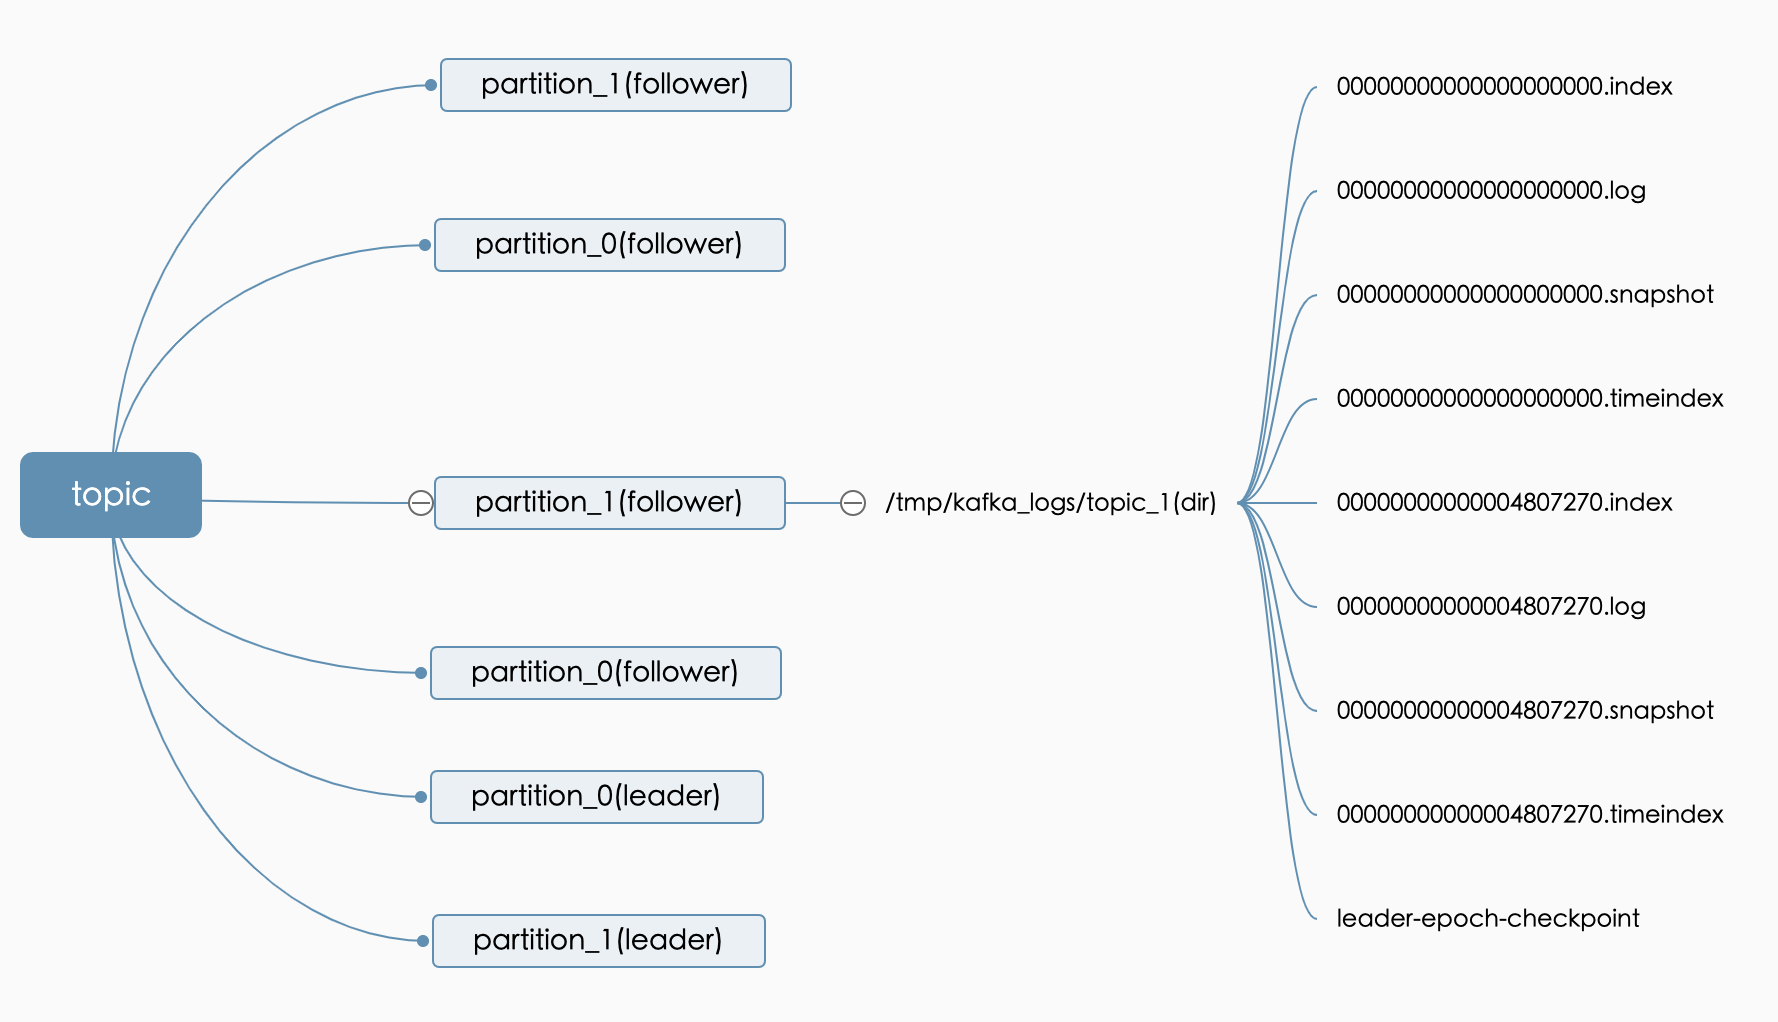
\includegraphics[width=0.9\linewidth]{image/0220}
        %\caption{}
        \label{fig:0220}
    \end{figure}
    
    
\end{frame}
\begin{frame}[plain,t]{Design} %也可以使用\frametitle{节的名字}效果一样
    \structure{The Consumer} \\
    \vspace{2ex}
    On each poll, consumer will try to use the last consumed offset as the starting offset and fetch sequentially. 
    
     \vspace{2ex}
    The last consumed offset can be manually set through seek(TopicPartition, long) or automatically set as the last committed offset for the subscribed list of partitions.
    
     \vspace{2ex}
    This method returns immediately if there are records available. Otherwise, it will await the passed timeout. If the timeout expires, an empty record set will be returned.
    
\end{frame}

\begin{frame}[plain,t]{Design} %也可以使用\frametitle{节的名字}效果一样
    \structure{The Consumer} \\
    \vspace{2ex}
    Our topic is divided into a set of totally ordered partitions, each of which is consumed by exactly one consumer within each subscribing consumer group at any given time。
    
    \begin{figure}
        \centering
        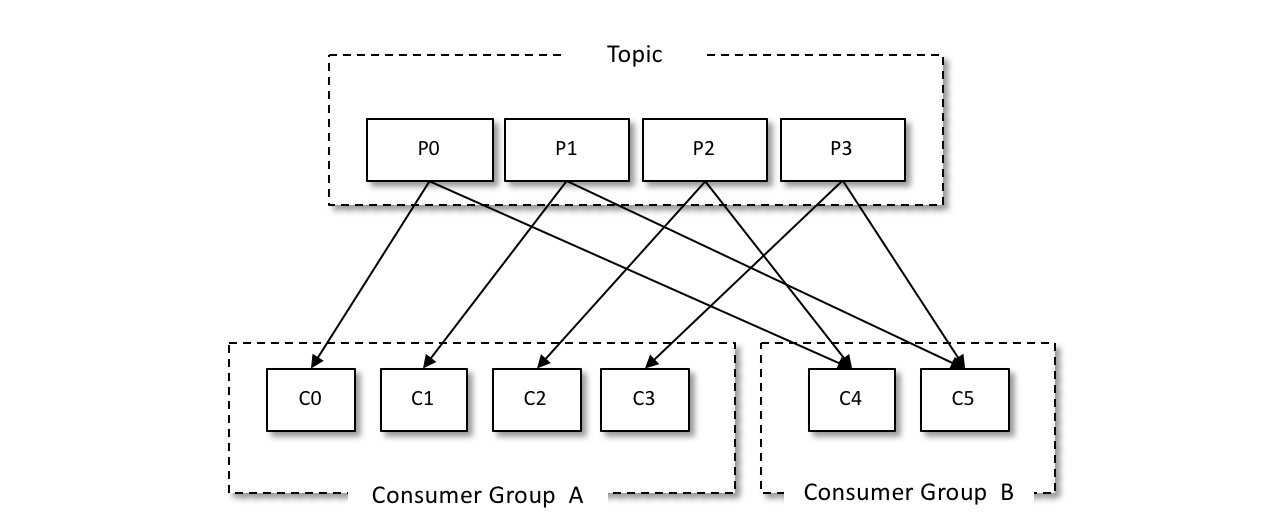
\includegraphics[width=0.9\linewidth]{image/0205}
        %\caption{}
        \label{fig:0205}
    \end{figure}
    
    
    
\end{frame}
\begin{frame}[plain,t]{Design} %也可以使用\frametitle{节的名字}效果一样
    \structure{The Consumer} \\
    %\vspace{2ex}
     \begin{figure}
        \centering
        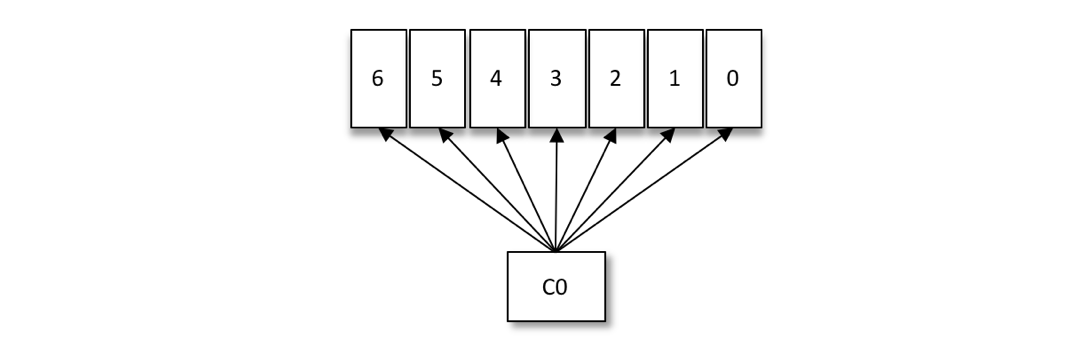
\includegraphics[width=0.9\linewidth]{image/0206}
        %\caption{}
        \label{fig:0206}
    \end{figure}
\vspace{-2ex}
 \begin{figure}
    \centering
    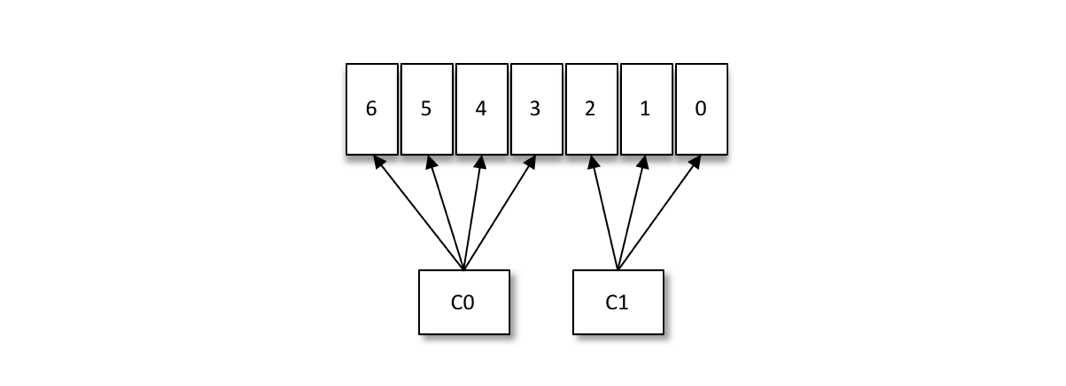
\includegraphics[width=0.9\linewidth]{image/0207}
    %\caption{}
    \label{fig:0207}
\end{figure}

    
    
    
\end{frame}
\begin{frame}[plain,t]{Design} %也可以使用\frametitle{节的名字}效果一样
    \structure{The Consumer} \\
    %\vspace{2ex}
       \begin{figure}
        \centering
        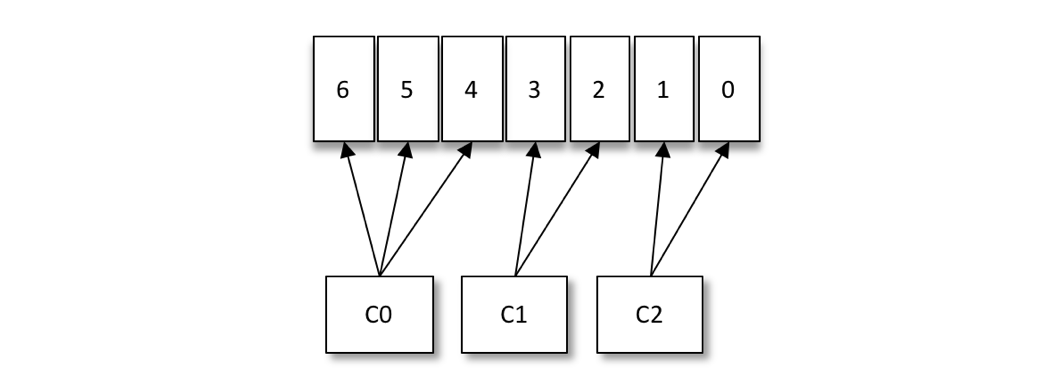
\includegraphics[width=0.9\linewidth]{image/0208}
        %\caption{}
        \label{fig:0208}
    \end{figure}
\vspace{-4ex}
    \begin{figure}
        \centering
        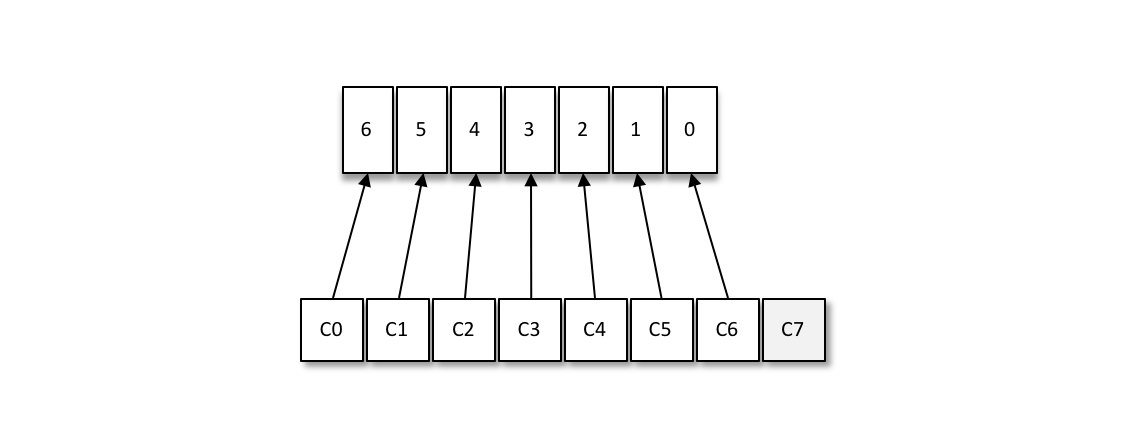
\includegraphics[width=0.9\linewidth]{image/0209}
        %\caption{}
        \label{fig:0209}
    \end{figure}
    
    
\end{frame}
\begin{frame}[plain,t]{Design} %也可以使用\frametitle{节的名字}效果一样
    \structure{The Consumer} \\
    \vspace{2ex}
    The rebalance protocol relies on the group coordinator to allocate entity ids to group members. 
    
     \vspace{2ex}
    These generated ids are ephemeral and will change when members restart and rejoin. 
    
     \vspace{2ex}
    Motivated by this observation, Kafka’s group management protocol allows group members to provide persistent entity ids(2.3+).
    
    
\end{frame}
\begin{frame}[plain,t]{Design} %也可以使用\frametitle{节的名字}效果一样
    \structure{The Consumer} \\
    \vspace{2ex}
   A Group Coordinator is a GroupMetadataManager and an Offset Manager,  at the same time.
   
   \begin{figure}
       \centering
       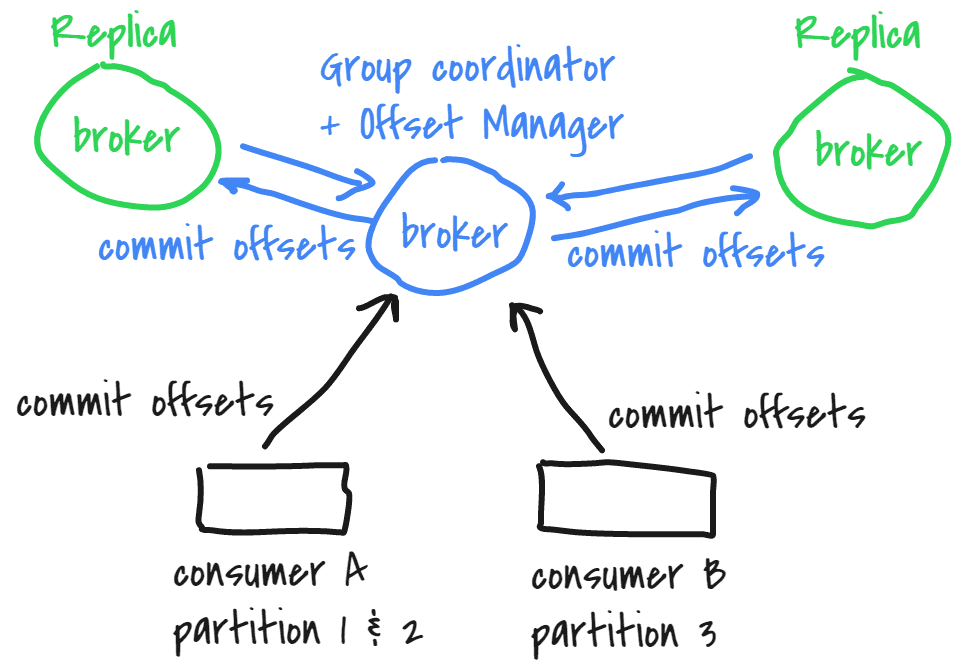
\includegraphics[width=0.7\linewidth]{image/0306}
       %\caption{}
       \label{fig:0306}
   \end{figure}
    
\end{frame}


\begin{frame}[plain,t]{Design} %也可以使用\frametitle{节的名字}效果一样
    \structure{The Consumer} \\
    \vspace{2ex}
   When the group coordinator receives an OffsetCommitRequest, it appends the request to a special compacted Kafka topic named \_\_consumer\_offsets.
   
   \vspace{2ex}
   It’s saved as binary data, each message in this topic has a key (group, topic, partition number) and a value.
   
    \vspace{2ex}
   
   \begin{figure}
       \centering
       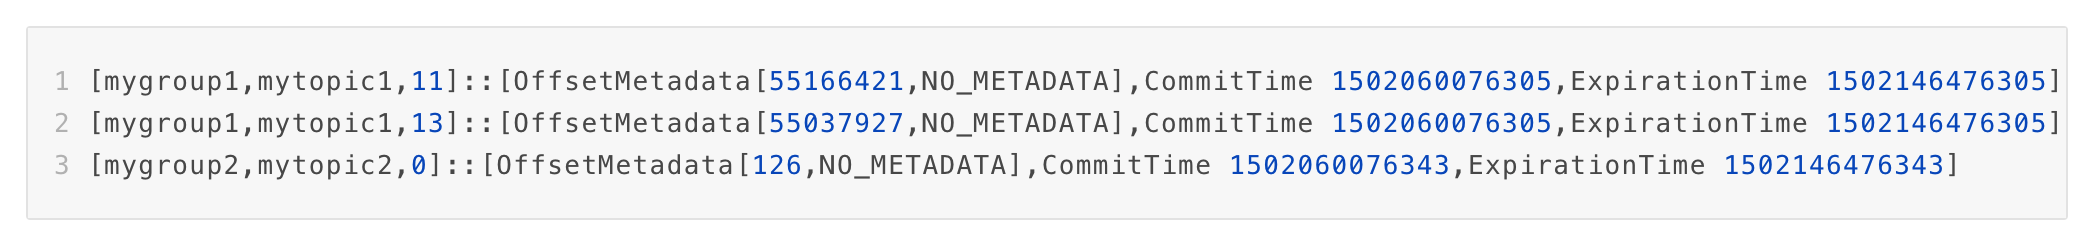
\includegraphics[width=1\linewidth]{image/0219}
       %\caption{}
       \label{fig:0219}
   \end{figure}
    
\end{frame}


\subsection{Message Delivery Semantics}
\begin{frame}[plain,t]{Design} %也可以使用\frametitle{节的名字}效果一样
    \structure{Message Delivery Semantics} \\
    \vspace{2ex}
    Let's discuss the semantic guarantees Kafka provides between producer and consumer.
    \begin{itemize}
        \item at most once
        \item at least once
        \item exactly once
    \end{itemize}

\vspace{2ex}
It's worth noting that this breaks down into two problems: the durability guarantees for publishing a message and the guarantees when consuming a message.
    
    
\end{frame}
\begin{frame}[plain,t]{Design} %也可以使用\frametitle{节的名字}效果一样
    \structure{Message Delivery Semantics} \\
    \vspace{2ex}
    When publishing a message we have a notion of the message being "committed" to the log. 
    
    \vspace{2ex}
    Once a published message is committed it will not be lost as long as one broker that replicates the partition to which this message was written remains "alive" (at least once). 
    
    \vspace{2ex}
    Since 0.11.0.0, the Kafka producer also supports an idempotent delivery option which guarantees that resending will not result in duplicate entries in the log (exactly once).
    
    
    
\end{frame}
\begin{frame}[plain,t]{Design} %也可以使用\frametitle{节的名字}效果一样
    \structure{Message Delivery Semantics} \\
    \vspace{2ex}
    The consumer controls its position in this log. 
    
    \vspace{2ex}
    It has several options for processing the messages and updating its position.
    
    \vspace{2ex}
    \begin{itemize}
        \item at least once (poll, update, process)
        \item at most once (poll, process, update)
        \item exactly once
        \begin{itemize}
            \item to topic (producer transactional capabilities)
            \item to external system (store offset in the same place as its output)
            
        \end{itemize}
    \end{itemize}
    
    
    
\end{frame}
\subsection{Replication}
\begin{frame}[plain,t]{Design} %也可以使用\frametitle{节的名字}效果一样
    \structure{Replication} \\
    \vspace{2ex}
    Kafka replicates the log for each topic's partitions across a configurable number of servers.
    
    %The unit of replication is the topic partition. 
    \vspace{2ex}
    Under non-failure conditions, each partition in Kafka has a single leader and zero or more followers
    
     \vspace{2ex}
    All reads and writes go to the leader of the partition.
    
    \begin{figure}
        \centering
        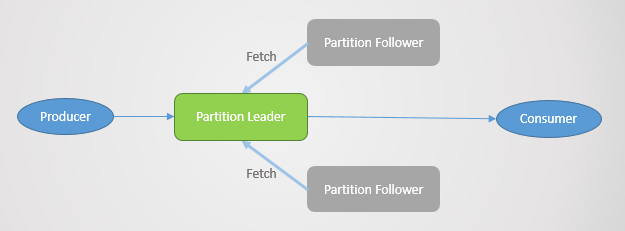
\includegraphics[width=0.9\linewidth]{image/0210}
        %\caption{}
        \label{fig:0210}
    \end{figure}
    
    

\end{frame}
\begin{frame}[plain,t]{Design} %也可以使用\frametitle{节的名字}效果一样
    \structure{Replication} \\
    \vspace{2ex}
    As with most distributed systems automatically handling failures requires having a precise definition of what it means for a node to be "alive". 
    
    \vspace{2ex}
    For Kafka node liveness has two conditions
    \begin{enumerate}
        \item  A node must be able to maintain its session with ZooKeeper (via ZooKeeper's heartbeat mechanism)
        \item If it is a follower it must replicate the writes happening on the leader and not fall "too far" behind
    \end{enumerate}
   
    
    
    
    
\end{frame}
\begin{frame}[plain,t]{Design} %也可以使用\frametitle{节的名字}效果一样
    \structure{Replication} \\
    \vspace{2ex}
    We refer to nodes satisfying these two conditions as being "in sync" to avoid the vagueness of "alive" or "failed". 
    
     \vspace{2ex}
    The guarantee that Kafka offers is that a committed message will not be lost, as long as there is at least one in sync replica alive, at all times.
    %The leader keeps track of the set of "in sync" nodes. 
    
    
    \begin{figure}
        \centering
        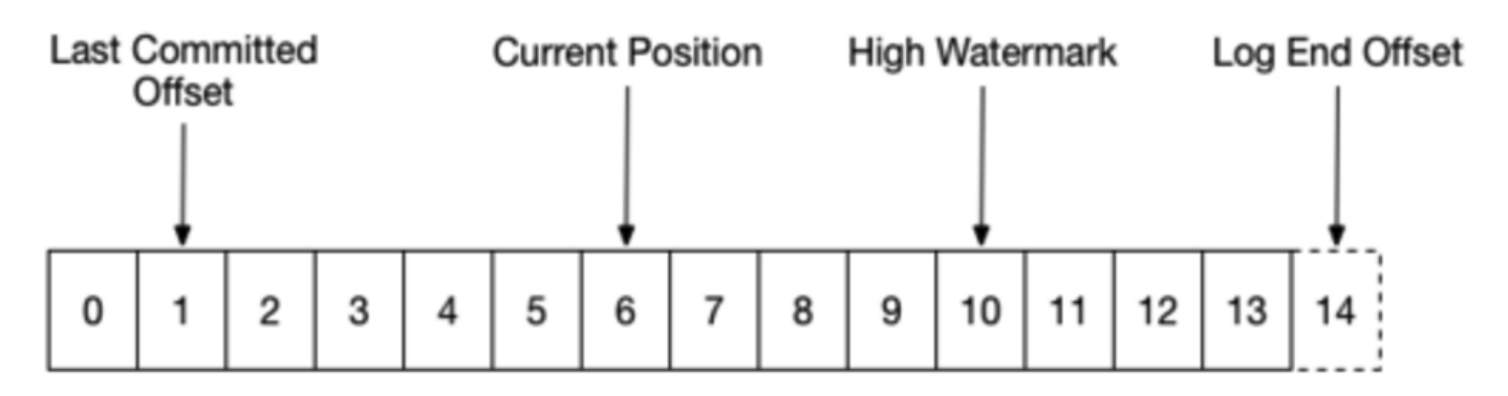
\includegraphics[width=0.9\linewidth]{image/0211}
        %\caption{}
        \label{fig:0211}
    \end{figure}
    
    

    
    
\end{frame}
\begin{frame}[plain,t]{Design} %也可以使用\frametitle{节的名字}效果一样
    \structure{Replication} \\
    \vspace{2ex}
    Instead of majority vote, Kafka dynamically maintains a set of in-sync replicas (ISR) that are caught-up to the leader. 
    
     \vspace{2ex}
    Only members of this set are eligible for election as leader. 
    
     \vspace{2ex}
    A write to a Kafka partition is not considered committed until all in-sync replicas have received the write. 
    
    
\end{frame}
\begin{frame}[plain,t]{Design} %也可以使用\frametitle{节的名字}效果一样
    \structure{Replication} \\
    \vspace{2ex}
    This ISR set is persisted to ZooKeeper whenever it changes. 
    
    \vspace{2ex}
    Because of this, any replica in the ISR is eligible to be elected leader. This is an important factor for Kafka's usage model where there are many partitions and ensuring leadership balance is important. 
    
    \vspace{2ex}
    With this ISR model and f+1 replicas, a Kafka topic can tolerate f failures without losing committed messages.
    
    
\end{frame}
\section{Implementation}
\subsection{Network Layer}
\begin{frame}[plain,t]{Implementation} %也可以使用\frametitle{节的名字}效果一样
    \structure{Network Layer} \\
    \vspace{2ex}
    The network layer is a fairly straight-forward NIO server.
    
    \vspace{2ex}
    The threading model is a single acceptor thread and N processor threads which handle a fixed number of connections each. 
    
    \vspace{1ex}
    \begin{figure}
        \centering
        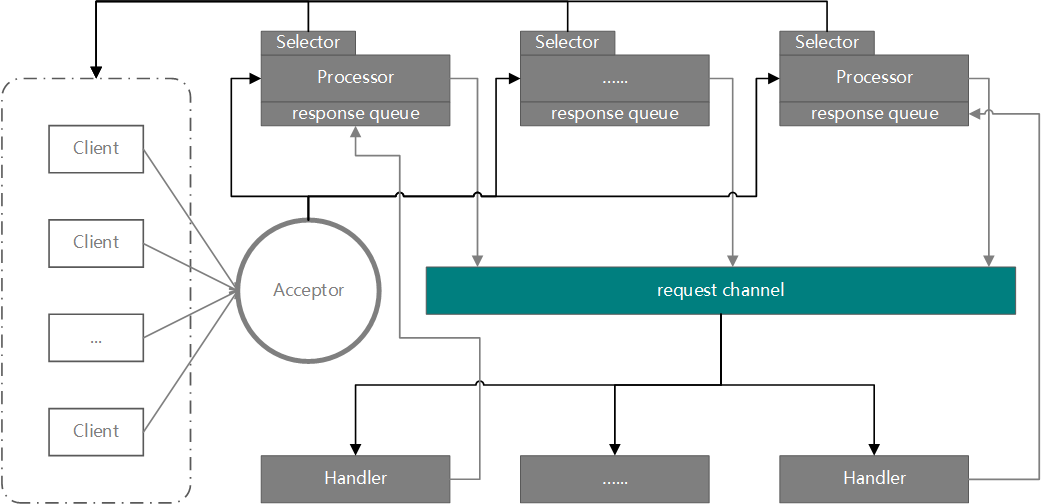
\includegraphics[width=0.9\linewidth]{image/0301}
        %\caption{}
        \label{fig:0301}
    \end{figure}
\end{frame}
\subsection{Messages}

\begin{frame}[plain,t]{Implementation} %也可以使用\frametitle{节的名字}效果一样
    \structure{Messages} \\
    \vspace{2ex}
    Messages consist of a variable-length header, a variable-length opaque key byte array and a variable-length opaque value byte array.
    
    \vspace{2ex}
    Leaving the key and value opaque enable user to choose a particular serialization type.
    
    \vspace{2ex}
    The RecordBatch interface is simply an iterator over messages with specialized methods for bulk reading and writing to an NIO Channel.
    
    
    
\end{frame}
\begin{frame}[plain,t]{Implementation} %也可以使用\frametitle{节的名字}效果一样
    \structure{Messages} \\
    \vspace{1ex}
    The following is the on-disk format of a RecordBatch.
    \vspace{-1ex}
    \begin{figure}
        \centering
        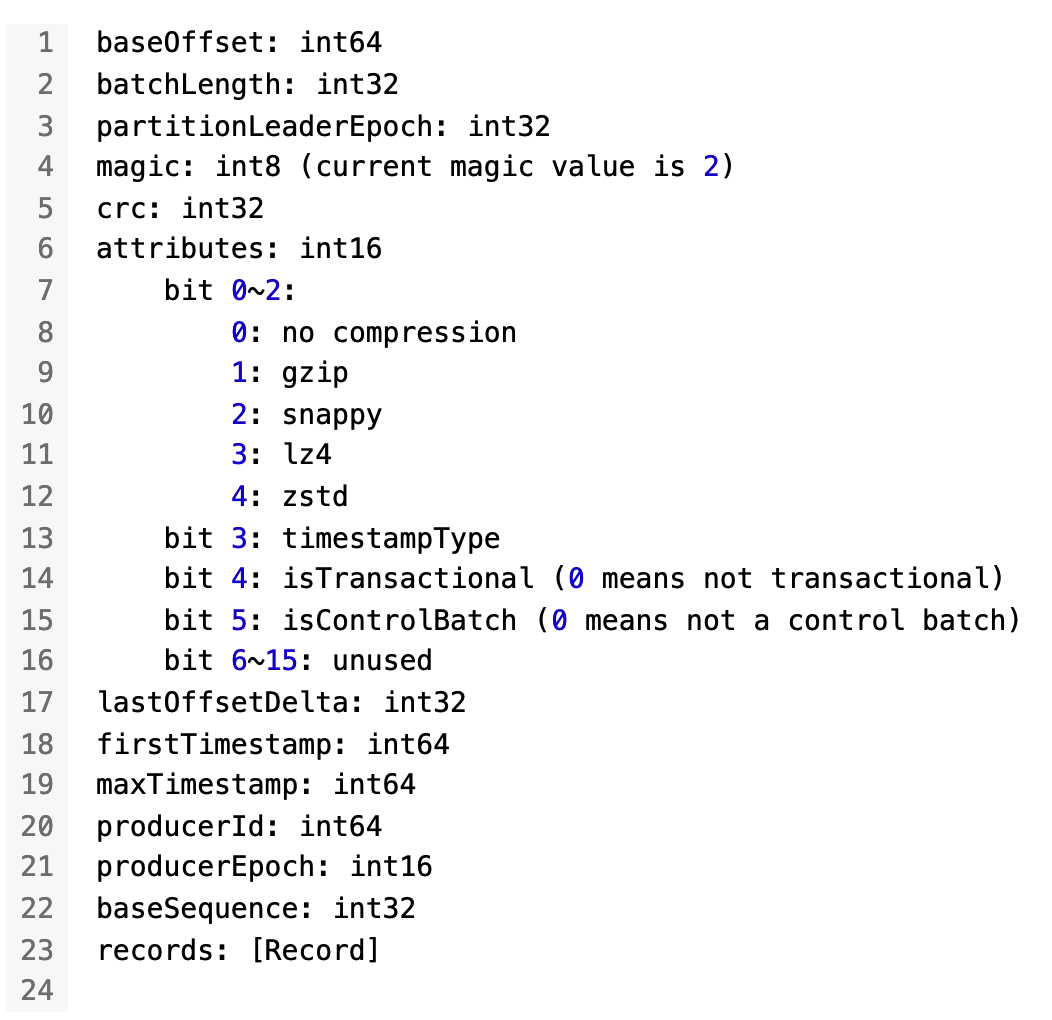
\includegraphics[width=0.7\linewidth]{image/0302}
        %\caption{}
        \label{fig:0302}
    \end{figure}
    
    
\end{frame}
\begin{frame}[plain,t]{Implementation} %也可以使用\frametitle{节的名字}效果一样
    \structure{Messages} \\
    \vspace{2ex}
    Record level headers were introduced in Kafka 0.11.0. The on-disk format of a record with Headers is delineated below.
    
    \vspace{2ex}
    \begin{figure}[htbp]
        \centering
        \begin{minipage}[t]{0.48\textwidth}
            \centering
                    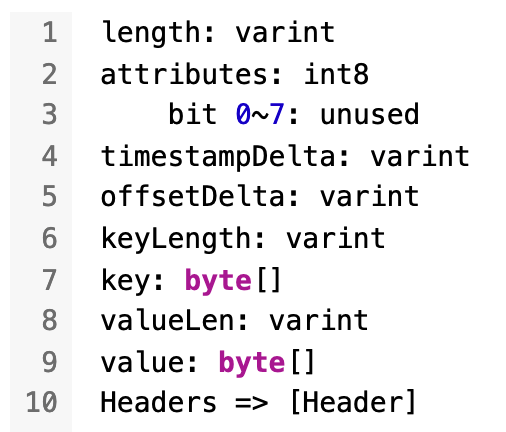
\includegraphics[width=0.8\linewidth]{image/0303}
            %\includegraphics[width=6cm]{test1.jpg}
            %\caption{World Map}
        \end{minipage}
        \begin{minipage}[t]{0.48\textwidth}
            \centering
                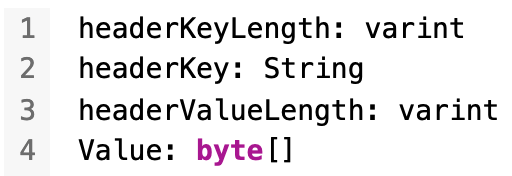
\includegraphics[width=0.8\linewidth]{image/0304}
            %\includegraphics[width=6cm]{test2.jpg}
            %\caption{Concrete and Constructions}
        \end{minipage}
    \end{figure}
    
   
  
    
\end{frame}
\subsection{Log}
\begin{frame}[plain,t]{Implementation} %也可以使用\frametitle{节的名字}效果一样
    \structure{Log} \\
    \vspace{2ex}
     Each log file is named with the offset of the first message it contains.
    \begin{figure}
        \centering
        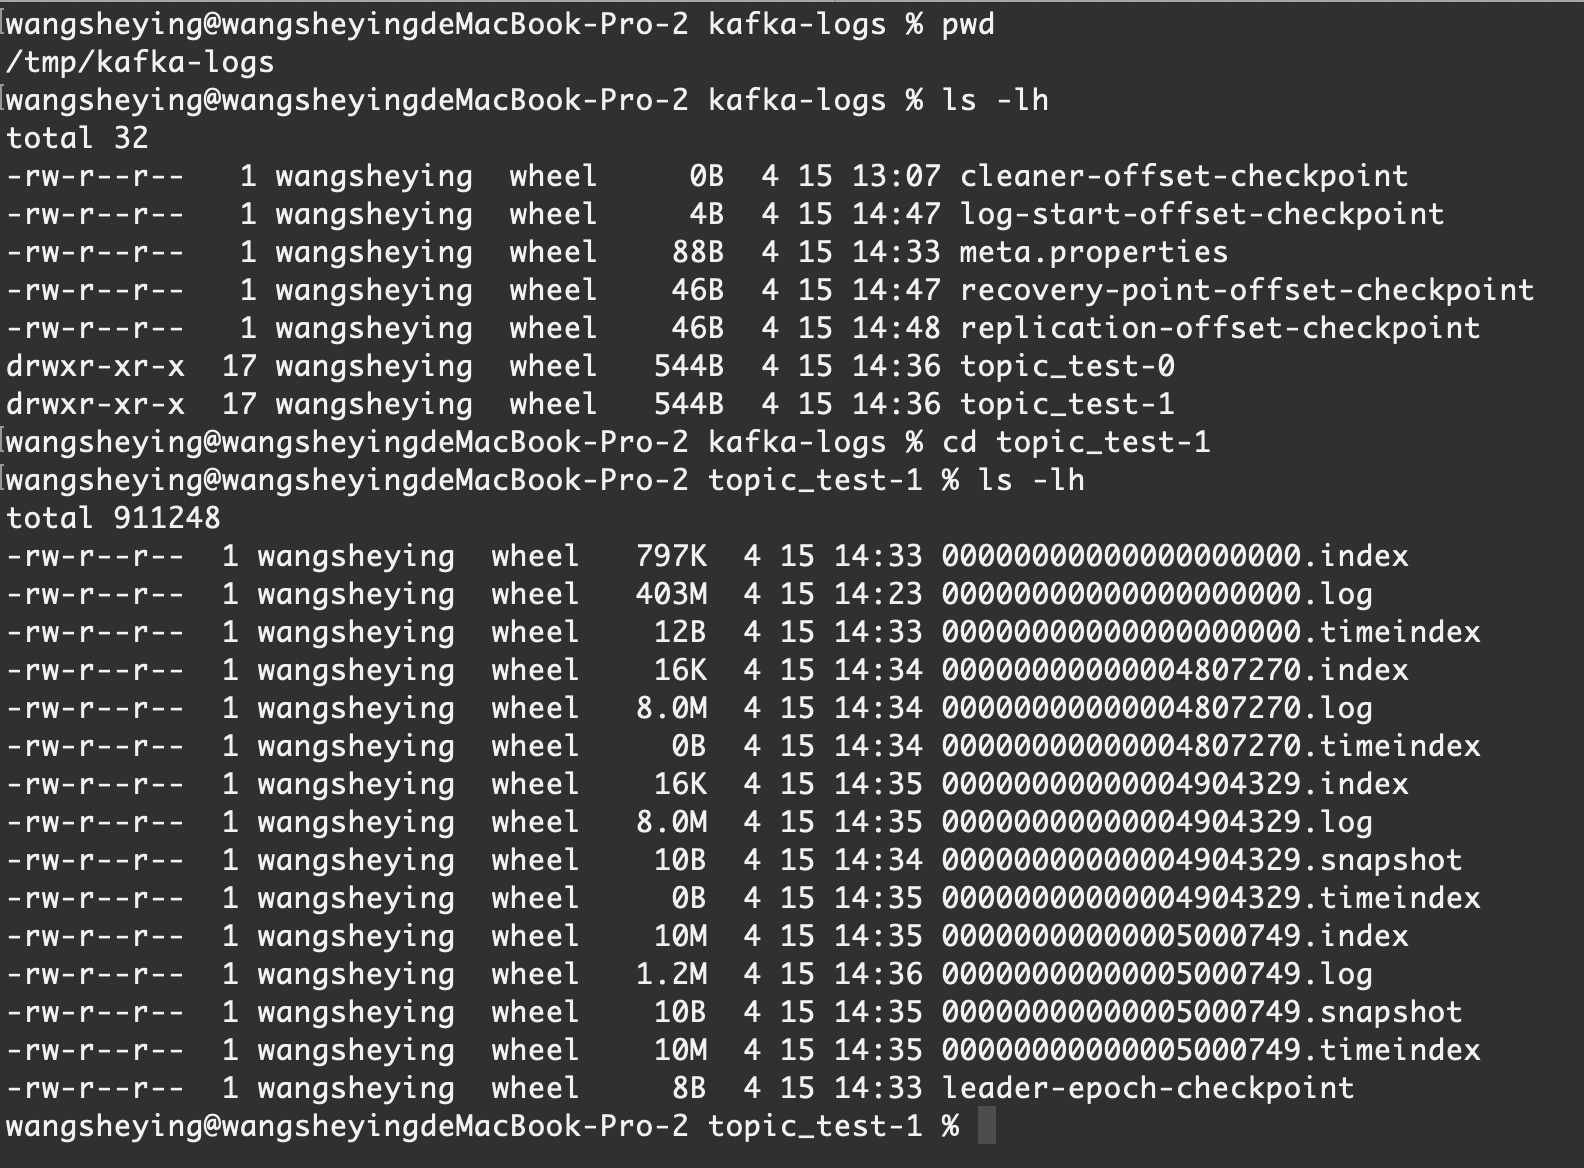
\includegraphics[width=0.8\linewidth]{image/0307}
        %\caption{}
        \label{fig:0307}
    \end{figure}
    
    
    
\end{frame}

\begin{frame}[plain,t]{Implementation} %也可以使用\frametitle{节的名字}效果一样
    \structure{Log} \\
    \vspace{2ex}
  The format of the log files is a sequence of "log entries""; each log entry is a 4 byte integer N storing the message length.
  
  \vspace{2ex}
  Each message is uniquely identified by a 64-bit integer offset giving the byte position of the start of this message in the stream of all messages ever sent to that topic on that partition.
    
    
     \vspace{2ex}
     The exact binary format for records is versioned and maintained as a standard interface so record batches can be transferred between producer, broker, and client without recopying or conversion when desirable.
    
    
    
\end{frame}

\begin{frame}[plain,t]{Implementation} %也可以使用\frametitle{节的名字}效果一样
    \structure{Log} \\
    \vspace{2ex}
    Reads are done by giving the 64-bit logical offset of a message and an S-byte max chunk size.
    
    \vspace{2ex}
    S is intended to be larger than any single message, but in the event of an abnormally large message, the read can be retried multiple times, each time doubling the buffer size, until the message is read successfully.
    
    \vspace{2ex}
    %It is likely that the read buffer ends with a partial message, this is easily detected by the size delimiting.
    The actual process of reading from an offset requires first locating the log segment file, calculating the file-specific offset from the global offset value, and then reading from that file offset. 
    
    
    
\end{frame}



%%=================================================================================================
\begin{frame}[plain]
    \huge
    \vfill
    \centerline{ \structure{Questions and Answers?} }
    \vfill
    
\end{frame}
\begin{frame}[plain]
    \huge
    \vfill
    \centerline{ \structure{Questions and Answers?} }
    \vfill
    \Huge
    \centerline{\alert{Thank You!} }
    \vfill
\end{frame}

%**********************************************************************************************
%                  上面就是正文,自己的内容
%        下面是标准的参考文献配置
%**********************************************************************************************
\begin{frame}[plain, t, allowframebreaks]{References}
    %  allowframebreaks,这个关键字可以使得参考文献自动断页,免得手动
    %  plain格式使得一帧的最上面是白色的,没有plain,会有色彩,可以试试
    %  t 使得正文不再是默认居中,而是在top,应该加上t,比较好看。
    \bibliographystyle{alpha}         %文献的格式apalike是[1],alpha是[Lam94]
    %\beamertemplatetextbibitems        %调整文献样式
    %\scriptsize                        %文献多时调整字体大小
    %\bibliography{math}                 %自己的文献
\end{frame}  
\end{document} 
%**********************************************************************************************
%        上面是标准的参考文献配置
%   参考文献的主题选择apalike,见《LaTeX入门》作者:刘海洋P423页(6-1-13)说明
%   apalike文献格式,按照美国心理协会(APA)的格式,提供基本的作者年代引用方式
%   避免完全不直观的数学编号可能造成的问题。这是因为beamer的文献格式比较特殊造成的
%  实例如下:
%\beamertemplatetextbibitems %该指令可使参考文献采用文字而不是图标的标注
%\begin{frame}[plain, t, allowframebreaks]{References}
%	\scriptsize
%	\bibliographystyle{apalike}
%	\bibliography{ZhangXiao-Smoothed_Analysis_of_Tensor_Decompositions} %文献命名规范,不要怕长
%\end{frame}

%**********************************************************************************************
%   学习LaTeX好的资料,有《LaTeX入门》《A Guide to LaTeX 4th Edition》 新浪微盘可下载  
%   《一份不太简短的LATEX介绍 》,网址 CTAN:/tex-archive/info/lshort 可下载  ,有中英文,每年更新
%   tex.stackexchange.com,一个美国的专业TeX问答网站,这个网站更灵活,受益匪浅
%   www.ctan.org            usepackage资料参考
%   www.texample.net       不常用,但是聚集了的专业绘图的LaTeX代码,比如画一个probability tree,
%   遇到问题,先百度Google,90%问题可解决,不行再上知乎提问,刘海洋老师,LaTeX专家,
%   可在 tex.stackexchange.com  同时提问,最基础的是读读上面的两本书,学会自己看文档
%   论文《Type setting mathematics for science and technology according to ISO 31/XI》
%   介绍排版中数学字体的选择
%***********************************************************************************************
